\documentclass{beamer}
\mode<presentation>
{
\usepackage{color}
\usepackage{graphicx}
\usepackage{tikz}
\usetheme[white]{Wisconsin}
\setbeamercovered{transparent}
}

\begin{document}

\title{DAGMC \& make\_watertight}
\author{Patrick C Shriwise}
\institute{University of Wisconsin - Madison}
\date{ December 06, 2013}

%--- Title Frame ------------%
\maketitle


%--- Frame 1 ----------------%
\begin{frame}
\frametitle{UW Fusion Neutronics Team}
\includegraphics[scale=0.65, trim = 0 0 20 0]{UWNeutronicsVenn.png}
\end{frame}

%--- Frame 2 ----------------%
\begin{frame}
\frametitle{Overview}

\begin{itemize}
\item Motivation
\item Developer's Perspective
	\begin{itemize}
	\item Core Software Infastructure
	\item Fundamental Geometry Operations
	\item Methods \& Accelerations
	\item Performance
	\end{itemize}
\item User's Perspective
	\begin{itemize}
	\item Workflow
	\item Examples
	\end{itemize}
\item Current Research
\end{itemize}
\end{frame}

%--- Frame 3 ----------------%
\begin{frame}
\frametitle{Motivation for CAD-based Monte Carlo}

\begin{itemize}
\item Faster
	\begin{itemize}
	\item faster design iteration
	\item provides a common domain inter-analysis coupling
	\end{itemize}
\item Cheaper
	\begin{itemize}
	\item reduced human effort
	\end{itemize}
\item Better
	\begin{itemize}
	\item avoidance of human error
	\item ability to describe higher-order surfaces
	\end{itemize}
\end{itemize}

\end{frame}



\end{document}


